
\section{Motivations behind Design Choices in ECT}
\label{sec:design-choices}

In this section, we expand upon our motivation behind the design decisions for the mapping function, metric, and weighting function used for ECT.

\paragraph{Mapping Function.}
We first assume that $\Delta t$ is \textit{approximately} proportional to $t$.
Let $0 < c \leq 1$ be this constant of proportionality, then we can write:
\begin{align*}
&c \approx \frac{\Delta t}{t} = \frac{t - r}{t} = 1 - \frac{r}{t} \Rightarrow
\frac{r}{t} \approx 1 - c.
\end{align*}

As training progresses, the mapping function should gradually shrink $\Delta t \to 0$. However, the above parameterization does not achieve this. An alternative parameterization is to decrease $\Delta t$ exponentially.
%
We assume the ratio between $r$ and $t$ can be written as:
%
\begin{equation}
\label{eq:const-mapping}
\frac{r}{t} = 1 - \frac{1}{q^a},
\end{equation}
%
where $q > 1$, $a = \lfloor\text{iters}/d\rfloor$, and $d$ is a hyperparameter controlling how quickly $\Delta t \to \d t$. At the beginning of training, $\frac{r}{t} = 1 - \frac{1}{q^0} = 0 \Rightarrow r = 0$, which falls back to DMs. Since we can initialize from the diffusion pretraining, this stage can be skipped by setting $a = \lceil\text{iters}/d\rceil$. As training progresses ($\text{iters} \uparrow$), $\frac{r}{t} \to 1$ leads to $\Delta t \to \d t$.

Finally, we adjust the mapping function to balance the prediction difficulties across different noise levels:
\begin{equation}
\label{eq:adj-mapping}
\frac{r}{t}
= 1 - \frac{1}{q^a} n(t)
= 1 - \frac{1}{q^{\lceil\text{iters}/d\rceil}} n(t).
\end{equation}
For $n(t)$, we choose $n(t) = 1 + k ,\sigma(-b,t) = 1 + \frac{k}{1 + e^{bt}}$, using the sigmoid function $\sigma$. Since $r\geq0$, we also clamp $r$ to satisfy this constraint after the adjustment.

\begin{figure}[htbp!]
    \vspace{10pt}
    \centering    
    \includegraphics[width=0.8\linewidth]{fig/mapping.pdf}
    \caption{Visualization of $\nicefrac{r}{t}$ during training. $\Delta t \to \d t$ when $\nicefrac{r}{t} \to 1$.}
    \label{fig:mapping}
\end{figure}
\vspace{0.3cm}

The intuition behind this mapping function is that the relative difficulty of predicting $f(\x_r)$ from $\x_t$ can vary significantly across different noise levels $t$ when using a linear mapping between $t$ and $r$.

Consider $\nicefrac{r}{t} = 0.9$. At small values of $t$, $\x_t$ and $\x_r$ are close, making the alignment of $f(\x_t)$ with $f(\x_r)$ relatively easy. In contrast, at larger $t$, where $\x_t$ and $\x_r$ are relatively far apart, the distance between the predictions $f(\x_t)$ and $f(\x_r)$ can be substantial. This leads to imbalanced gradient flows across different noise levels, impeding the training dynamics.

Therefore, we downscale $\nicefrac{r}{t}$ when $t$ is near $0$ through the mapping function, balancing the gradient flow across varying noise levels. 
This prevents the gradient at any noise level from being too small or too large relative to other noise levels, thereby controlling the variance of the gradients. 

We direct the reader to \cref{sec:additional-experimental-results} for details of how to set $q^{\lceil\text{iters}/d\rceil}$.

\paragraph{Choice of Metric.}
As discussed in \cref{sec:preliminaries}, iCT uses pseudo-Huber metric~\citep{huber} to mitigate the perceptual bias caused by the LPIPS metric~\citep{lpips}, 
\begin{align}
L(\x, \y) = \sqrt{\| \x - \y \|_2^2 + \epsilon} - \epsilon, \quad \epsilon > 0.
\end{align}
%
This metric indeed improves the performance of CMs over the classic squared $L_2$ loss. When taking a careful look as this metric, we reveal that one of the reasons for this improvement is that this metric is more robust to the outliers compared to the $L_2$ metric due to its adaptive per-sample scaling of the gradients.
Let $\Delta = \x - \y$, then the differential of the pseudo-Huber metric can be written as
%
\begin{equation}
\label{eq:grad-huber}
\mathrm{d} L = \underbrace{\frac{1}{\sqrt{\|\Delta\|_2^2 + c^2}} \vphantom{\mathrm{d} \left( \frac{1}{2} \|\Delta\|_2^2 \right)} }_{\text{weighting term}} \underbrace{\mathrm{d} \left( \frac{1}{2} \|\Delta\|_2^2 \vphantom{\frac{1}{\sqrt{\|\Delta\|_2^2 + \epsilon}}}\right)}_{\text{differential of 
 squared } L_2 \text{\,loss}},
\end{equation}
%
where we have decomposed the differential of pseudo-Huber loss into an adaptive weighting term and the differential of the squared $L_2$ loss.
Therefore, we retain the squared $L_2$ metric used in DMs, and explore varying adaptive weighting terms which we explore in detail in \cref{sec:additional-experimental-results}.

\paragraph{Distinction between the training schedules of ECT and iCT.} 
As noted in \cref{sec:preliminaries}, iCT \citep{ict} employs a discrete-time curriculum given by ~\cref{schedule}. 
This curriculum divides the noise horizon $[0,T]$ into $N$ smaller consecutive subintervals to apply the consistency loss, characterized by non-overlapping segments $[t_i, t_{i+1}]$, and gradually increases the number of intervals $N=10 \to 1280$. 
%
However, the "boundary" condition of this schedule is to start with the number of intervals to $N=1$, learning a model solely mapping samples at noise levels $T_{\text{max}}$ to the clean data $\x_0$, largely distinct from the classic diffusion models training.
%
We instead investigate a continuous-time schedule whose "boundary" condition yields diffusion pretraining, \ie constructing training pairs of $r=0$ for all $t$ at the beginning.

% We propose a vastly different continuous-time training schedule that aids in mitigating the "curse of consistency" as discussed in \cref{sec:tacking-curse-of-consistency}.

\section{Exploring Design Space \& Scaling of Consistency Models}
\label{sec:additional-experimental-results}

Due to ECT's efficiency, we can explore the design space of CMs at a minimal cost. We specifically examine the weighting function, training schedule, and regularization for CMs.

Our most significant finding is that \textit{controlling gradient variances and balancing the gradients across different noise levels are fundamental to CMs' training dynamics}. Leveraging the deep connection between CMs and DMs, we also improve the diffusion pretraining and the full pretraining+tuning pipeline using our findings.

\paragraph{Weighting Function.} Forward processes with different noise schedules and model parameterizations can be translated into each other at the cost of varying weighting functions~\citep{wt}.
From our experiments on a wide range of weighting schemes, we learn three key lessons.

\begin{table}[t!]
\vspace{5pt}
\caption{Performance of ECMs trained with various weighting functions on \imgnet. We enable the adaptive weighting $w(\Delta) = \nicefrac{1}{(\|\Delta\|_2^2 + c^2)^{\frac{1}{2}}}$.}
\vspace{5pt}
\centering
\begin{tabular}{@{}lcc@{}} 
\toprule
$\Bar{w}(t)$ & 1-step FID$\downarrow$ & 2-step FID$\downarrow$ \\ 
\midrule
$1$                   & \textbf{5.39}   & 3.48  \\
$\nicefrac{1}{t}$     & 17.79	        & 3.24  \\
$\nicefrac{1}{(t-r)}$ & 9.28	        & 3.22  \\
$\nicefrac{1}{t}+\nicefrac{1}{\sigma_{\mathrm{data}}}$  & 5.68 & 3.44  \\
$\nicefrac{1}{t^2}$   & 190.80          & 20.65         \\
$\nicefrac{1}{t^2}+1$ & 6.78            & \textbf{3.12} \\
$\nicefrac{1}{t^2}+\nicefrac{1}{\sigma_{\mathrm{data}}^2}$ & 5.51 & 3.18 \\
$\nicefrac{1}{(t^2 +\sigma_{\mathrm{data}}^2)}$ & 163.01          & 13.33 \\
\bottomrule
\end{tabular}
\label{tab:wt-imgnet}
\end{table}

$(1)$ \textit{There is no free lunch for weighting function}, \ie there is likely no universal timestep weighting $\Bar{w}(t)$ that can outperform all other candidates on different datasets, models, and target metrics for both 1-step and 2-step generation. 

We refer these results to \cref{tab:wt-imgnet}, including $\mathrm{SNR}(t) = \nicefrac{1}{t^2}$, $\mathrm{SNR}(t)+1 = \nicefrac{1}{t^2}+1$~\citep{salimans2022progressive}, EDM weighting $\mathrm{SNR}(t) + \nicefrac{1}{\sigma_{\mathrm{data}}^2} = \nicefrac{1}{t^2}+\nicefrac{1}{\sigma_{\mathrm{data}}^2}$~\citep{Karras2022edm}, and Soft-Min-SNR weighting $\nicefrac{1}{(t^2 +\sigma_{\mathrm{data}}^2)}$~\citep{min-snr,soft_min_snr}, where $\mathrm{SNR}(t) = \nicefrac{1}{t^2}$ is the signal-to-noise ratio in our setup.

On CIFAR-10, the weighting $\Bar{w}(t) = \nicefrac{1}{(t-r)}$ from the discretization of consistency condition in \cref{eq:CMcost} achieves the best 1-step FID, while the square root of $\mathrm{SNR}(t)$, $\Bar{w}(t) = \sqrt{\mathrm{SNR}(t)} = \nicefrac{1}{t}$, produces the best \dino. 
On \imgnet, considering that we have already had the adaptive weighting $w(\Delta)$, the uniform weighting $\Bar{w}(t) \equiv 1$ can demonstrate the best 1-step FID when tuning from EDM2~\citep{Karras2024edm2}.
%
In contrast to 1-step FIDs, a wider range of timestep weighting $\Bar{w}(t)$ produces close 2-step FIDs for ECMs. 

When starting on a new dataset with no prior information, $\Bar{w}(t) = \mathrm{SNR}(t)+n$ is a generally strong choice as the default timestep weighting of data prediction models (x-pred). In this situation, this weighting function corresponds to using v-pred~\citep{salimans2022progressive} or flow matching~\citep{lipman2022flow,liu2022flow} as model parameterization when $n=1$.

\begin{table}[t!]
\caption{Performance of ECMs trained with varying adaptive weightings on \imgnet.}
\vspace{5pt}
\centering
\begin{tabular}{@{}llcc@{}} 
\toprule
$\Bar{w}(t)$ & $w(\Delta)$ & 1-step FID$\downarrow$ & 2-step FID$\downarrow$ \\ 
\midrule
$\nicefrac{1}{t^2}+\nicefrac{1}{\sigma_{\mathrm{data}}^2}$ & $1$ & 6.51   & 3.28     \\
$\nicefrac{1}{t^2}+\nicefrac{1}{\sigma_{\mathrm{data}}^2}$ & $\nicefrac{1}{(\|\Delta\|_1 + c})$          & 6.29	 & 3.25	 \\
$\nicefrac{1}{t^2}+\nicefrac{1}{\sigma_{\mathrm{data}}^2}$ &  $\nicefrac{1}{(\|\Delta\|_2^2 + c^2)^{\frac{1}{2}}}$ & 5.51   & 3.18     \\
$1$ & $\nicefrac{1}{(\|\Delta\|_2^2 + c^2)^{\frac{1}{2}}}$ &  5.39  & 3.48 \\
\bottomrule
\end{tabular}
\label{tab:adaptive-wt-imgnet}
\end{table}
\vspace{0.2cm}

$(2)$ \textit{The adaptive weighting $w(\Delta)$ achieves better results by controlling gradient variance}. The adaptive weighting $w(\Delta)$ on a per-sample basis shows uniform improvements on both CIFAR-10 and \imgnet. See \cref{tab:adaptive-wt-imgnet} for the ablation study. 

Beyond ECT, we further investigate the role of adaptive weighting \( w(\Delta) \) in pretraining on a toy Swiss roll dataset using the parameterization and forward process of flow matching~\citep{lipman2022flow} and an MLP network.

Consider the objective function \( w(\Delta) \|v_\theta(\x_t) - (\x_1 - \x_0) \|_2^2 \), where \( \x_t = (1-t) \cdot \x_0 + t \cdot \x_1 \), \(t \sim \mathrm{Uniform}(0, 1)\), \( \x_1 \sim \mathcal{N}(\mathbf{0}, \mathbf{I})\), and the adaptive weighting
\[
w(\Delta) = \frac{1}{(\|\Delta\|_2^2 + \epsilon)^p},
\]
where \( p=0 \) corresponds to no adaptive weighting. We set \( \epsilon = 10^{-6} \) and control the strength of gradient normalization by varying \( p \) from $0$ to $1$.

As we increase the strength of adaptive weighting, flow models become easier to sample from in a few steps. Surprisingly, even \( p=1 \) demonstrates strong few-step sampling results when pretraining the flow model. See \cref{fig:adp-wt} for visualization.

% $(3)$ \textit{The timestep weighting $\Bar{w}(t)$ and the adaptive weighting $w(\Delta)$ are compatible}. This compatibility is how we build ECMs in this work, using adaptive weighting \( w(\Delta) \) to achieve strong 1-step sampling capabilities and timestep weighting \( \Bar{w}(t) \) to improve 2-step sampling.

\paragraph{Mapping Function.} We compare the constant mapping function with $n(t) \equiv 1$ in \cref{eq:const-mapping} and mapping function equipped with the sigmoid $n(t)$ in \cref{eq:adj-mapping}. We use $k=8$ and $b=1$ for all the experiments, which transfers well from CIFAR-10 to \imgnet\ and serves as a baseline in our experiments. Though $b=2$ can further improve the 1-step FIDs on \imgnet, noticed post hoc, we don't rerun our experiments.

\begin{figure}[t!]
    \vspace{10pt}
    \centering 
    \includegraphics[width=0.8\linewidth]{fig/adp_wt_order.pdf}
    \caption{Influence of adaptive weighting $w(\Delta) = \nicefrac{1}{(\|\Delta\|_2^2 + \epsilon)^p}$ on pretraining using varying $p$.}
    \label{fig:adp-wt}
    \vspace{-10pt}
\end{figure}
On CIFAR-10, the constant mapping function with $n(t) \equiv 1$ achieves 1-step FID of 4.06 at $200$k iterations, worse than the 1-step FID of 3.86 by $n(t)= 1 + \frac{k}{1 + e^{bt}}$.
Under our forward process ($\x_t = \x_0 + t \cdot \epsilon$) and model parameterization (EDM~\citep{Karras2022edm}), the constant mapping function incurs training instability on \imgnet, likely due to the imbalanced gradient flow. 

The role of the mapping function, regarding training, is to balance the difficulty of learning \textit{consistency condition} across different noise levels, avoiding trivial consistency loss near $t \to 0$.
%
For model parameterizations and forward processes different from ours, for example, flow matching~\citep{lipman2022flow,liu2022flow,sd3}, we advise readers to start from the constant mapping function due to its simplicity.

\vspace{-10pt}
\paragraph{Dropout.} In line with \citep{ict}, we find that CMs benefit significantly from dropout~\citep{dropout}.  
On CIFAR-10, we apply a dropout of $0.20$ for models evaluated on FID and a dropout of $0.30$ for models evaluated on \dino. 

On \imgnet, we note that ECT benefits from a surprisingly high dropout rate. When increasing the dropout rate from $0.10$ to $0.40$, the 2-step FID decreases from $4.53$ to $3.24$. 
Increasing the dropout rate further can be helpful for 1-step FID under certain timestep weighting $\Bar{w}(t)$, but the 2-step FID starts to deteriorate.
In general, we optimize our model configurations for 2-step generation and choose the dropout rate of $0.40$ for ECM-S.

Finally, we note that the dropout rate tuned at a given weighting function $w(t)$ transfers well to the other weighting functions, thereby reducing the overall cost of hyperparameter tuning. 
On \imgnet, the dropout rate can even transfer to different model sizes. We apply a dropout rate of $0.50$ for all the model sizes of ECM-M/L/XL.


\paragraph{Shrinking $\Delta t \to \mathrm{d}t$.} 
In the mapping function discussed in \cref{sec:ect} and \cref{sec:design-choices}, we use the hyperparameter $d$ to control the magnitude of $q$, thereby determining the overall rate of shrinking $\Delta t \to \mathrm{d}t$, given by $\left(1 - \nicefrac{1}{q}^{\lceil\text{iters}/d\rceil} \right)$.
In practice, we set $q=2$ and $d = \text{total\_iters}//8$ for CIFAR-10 experiments, and $q=4$ and $d = \text{total\_iters}//4$ for \imgnet\ experiments, achieving $\nicefrac{r}{t} \approx 0.99$ at the end of training.

Compared with no shrinkage of $\Delta t$, where $\Delta t \approx \mathrm{d}t$ throughout, we find that shrinking $\Delta t \to \mathrm{d}t$ results in improved performance for ECMs. 
%
For example, on CIFAR-10, starting ECT directly with $\Delta t \approx \mathrm{d}t$ by setting $q=256$ (corresponding to $\nicefrac{r}{t} \approx 0.99$) leads to quick improvements in sample quality initially but slower convergence later on. The 1-step FID drops from 3.60 to 3.86 using the same 400k training iterations compared to gradually shrinking $\Delta t \to \mathrm{d}t$. 
%
On \imgnet, $\Delta t \approx \mathrm{d}t$ with $q=256$ from the beginning results in training divergence, as the gradient flow is highly imbalanced across noise levels, even when initializing from pretrained diffusion models.

This observation suggests that \emph{ECT's schedule should be adjusted according to the compute budget}. At small compute budgets, as long as training stability permits, directly approximating the \textit{differential consistency condition} through a small $\Delta t \approx \mathrm{d}t$ leads to fast sample quality improvements. For normal to rich compute budgets, shrinking $\Delta t \to \mathrm{d}t$ generally improves the final sample quality, which is the recommended practice.

Using this feature of ECT, we demonstrate its efficiency by training ECMs to surpass previous Consistency Distillation, which took hundreds of GPU hours, using \textcolor{tomato}{\textbf{one hour on a single A100 GPU}}.

\paragraph{Training Generative Models in 1 GPU Hour.} Deep generative models are typically computationally expensive to train. Unlike training a classifier on CIFAR-10, which usually completes within one GPU hour, leading generative models on CIFAR-10 as of 2024 require days to a week to train on 8 GPUs. Even distillation from pretrained diffusion models can take over a day on 8 GPUs or even more, equivalently hundreds of GPU hours.

To demonstrate the efficiency of ECT and facilitate future studies, we implemented a fast prototyping setting designed to yield results within one hour on a single GPU. This configuration uses a fixed $\Delta t \approx \mathrm{d}t$ by setting $q=256$ in our mapping function (corresponding to $\frac{r}{t} \approx 0.99$), which allows for quick approximation of the differential consistency condition.  Through $8000$ gradient descent steps at batch size of $128$, within 1 hour on a single A100 40GB GPU, ECT achieves a 2-step FID of $2.73$, outperforming Consistency Distillation (2-step FID of $2.93$) trained with 800k iters at batch size 512 and LPIPS~\citep{lpips} metric.

% \section{Ablation Study}

\paragraph{Ablation on Pretraining}
We conducted a controlled experiment, training CMs from scratch following iCT best practices and tuning EDM using both iCT and ECT schedules. The combined pretraining and fine-tuning cost for ECT is $50\% + 6.25\%$ of iCT trained from scratch. Results are presented in \cref{tab:pretraining-impact}.

There is a noticeable performance gap between iCT's training and ECT's pretraining+tuning scheme, particularly when evaluating models using modern metrics like $\mathrm{FD}_{\text{DINOv2}}$~\citep{fd_dino}.  $\mathrm{FD}_{\text{DINOv2}}$ employs the representation space of the DINOv2-L model~\citep{oquab2023dinov2} to compute distributional distance, which has been shown to better align with human evaluations.

\begin{table}[h]
\centering
\caption{Impact of pretraining on model performance}
\vspace{5pt}
\label{tab:pretraining-impact}
\begin{tabular}{lc}
\toprule
Model & $\mathrm{FD}_{\text{DINOv2}}$ \\
\midrule
iCT                       & 242.30 \\
Pretraining + iCT tuning  & 200.31 \\
Pretraining + ECT tuning  & 190.13 \\
EDM                       & 168.16 \\
\bottomrule
\end{tabular}
\vspace{10pt}
\end{table}

When scaling up the pretraining+tuning cost to match the overall cost of iCT in class-conditional settings, ECM achieves a $\mathrm{FD}_{\text{DINOv2}}$ of 152.21, significantly outperforming the iCT model trained from scratch (205.11). For context, StyleGAN-XL achieves an $\mathrm{FD}_{\text{DINOv2}}$ of 204.60.

\begin{table}[t!]
\caption{Generative performance on class-conditional CIFAR-10. }
\vspace{5pt}
\centering
\small
\centering
\setlength{\tabcolsep}{5pt} % Adjust horizontal padding between columns
\renewcommand{\arraystretch}{0.98} % 
\begin{tabular}{@{}lccc@{}}
\toprule
Method & \dino$\downarrow$ & NFE$\downarrow$ \\ 
\midrule
{\color{gray} GANs} & ~ & ~ \\ 
\midrule
BigGAN~\citep{biggan}               & 326.66 & 1 \\
StyleGAN2-ADA~\citep{Karras2020ada} & 305.92 & 1 \\
StyleGAN-XL~\citep{styleganxl}      & 204.60 & 1 \\
\midrule
{\color{gray} Diffusion Models} & ~ & ~ \\ 
\midrule
EDM~\citep{Karras2022edm}	& 145.20 & 35 \\
PFGM++~\citep{xu2023pfgm++}  & 141.65 & 35 \\
\midrule
{\color{gray} ECT} & ~ & ~ \\ 
\midrule
ECM (ECT Pretrained) & 121.05 & 35\\
ECM (Tuned) & 198.51 & 1 \\
ECM	(Tuned) & 128.63 & 2 \\
\bottomrule
\end{tabular}
\label{tab:cifar-dino}
\end{table}

\paragraph{Ablation on Tuning Design Choices}
Besides quantitatively evaluating the pretraining impact, we conduct further ablation studies regarding fine-tuning design choices. Due to the computational constraints, we tune EDM2-S using iCT's design choices as the baseline.  Results are presented in \cref{tab:tuning-ablation}. These results demonstrate the improvements of the continuous-time training schedule, increased dropout, and weighting functions on ECMs' generative performance.

\begin{table}[h]
\centering
\caption{Ablation study of continuous-time CMs on \imgnet}
\vspace{5pt}
\label{tab:tuning-ablation}
\begin{tabular}{lcc}
\toprule
Methods & 1-step FID & 2-step FID \\
\midrule
iCT + EDM2 Pretraining                             & 21.09 & 4.39 \\
+ Continuous-time schedule                         & 14.34 & 4.33 \\
+ Dropout = 0.40                                   & 9.28  & 3.22 \\
+ $\Bar{w}(t)=\nicefrac{1}{t^2}+\nicefrac{1}{\sigma_{\mathrm{data}}^2}$ & 5.51  & 3.18 \\
\bottomrule
\end{tabular}
\vspace{5pt}
\end{table}


\paragraph{Improving Pretraining using Findings in Tuning.} The exploration of the design space through the tuning stage as a proxy led to a question: Can the insights gained during tuning be applied to improve the pretraining stage and, consequently, the entire pretraining+tuning pipeline for CMs? The results of our experiments confirmed this hypothesis.

For the largest $\Delta t = t$, ECT falls back to diffusion pretraining with $r=0$ and thus $\f(\x_r) = \x_0$. 
%
We pretrain EDM~\citep{Karras2022edm} on the CIFAR-10 dataset using the findings in ECT. Instead of using EDM weighting, $\mathrm{SNR}(t) + \nicefrac{1}{\sigma_{\mathrm{data}}^2}$, we enable the adaptive weighting $w(\Delta)$ with $p=\nicefrac{1}{2}$ and smoothing factor $c=0$ and a timestep weighting $\Bar{w}(t) = \nicefrac{1}{t}$.

Compared with the EDM baseline, the recipe from ECT brings a convergence acceleration over $2\times$ regarding \dino, matching EDM's final performance using less than half of the pretraining budget and largely outperforming it at the full pretraining budget. 

EDM pretrained by ECT achieves \dino\ of $150.39$ for unconditional generation and $121.05$ for class-conditional generation, considerably better than the EDM baseline's \dino\ of $168.17$ for unconditional generation and $145.20$ for class-conditional generation, when using the same pretraining budget and inference steps (NFE=35).

\paragraph{Influence of Pretraining Quality.} Using ECT pretrained models (\dino\ of $121.05$) and original EDM~\citep{Karras2022edm} (\dino\ of $145.20$), we investigate the influence of pretraining quality on consistency tuning and resulting ECMs.
%
Our experiments confirm that better pretraining leads to easier consistency tuning and faster convergence.
At the same budget of $204.8\mathrm{M}$ images, tuning from ECT pretrained models achieves \dino\ of $128.63$, better than \dino\ of $152.21$ from EDM. 

ECM from the ECT pretraining surpasses SoTA GANs in 1 sampling step and advanced DMs in 2 sampling steps, only slightly falling behind our pretrained models and setting up a new SoTA for the modern metric \dino. Results can be found in \cref{tab:cifar-dino}. 

On \imgnet, ECM-M, initialized from EDM2-M~\citep{Karras2024edm2}, deviates from the power law scaling and achieves better generative performance than the log-linear trend. (See \cref{fig:imgnet-scaling}, Right). We speculate that it is due to a higher pretraining budget, in which EDM2-M was pretrained by $2\times$ training images compared with other model sizes (S/L/XL).

\paragraph{Differences between 1-step and 2-step Generation.}
%
Our empirical results suggest that the training recipe for the best 1-step generative models can differ from the best few-step generative models in many aspects, including weighting function, dropout rate, and EMA rate/length.
%
\cref{fig:fid-dropout-nfe} shows an example of how FIDs from different numbers of function evaluations (NFEs) at inference vary with dropout rates. 

In our setups, starting from a proper model size, the improvements from 2-step sampling seem larger than doubling the model size but keeping 1-step sampling.
In the prior works, iCT~\citep{ict} employs $2\times$ deeper model, but the 1-step generative performance can be inferior to the 2-step results from ECT. 
%
This finding is consistent with recent theoretical analysis \citep{lyu2023convergence}, which indicates a tighter bound on the sample quality for the 2-step generation compared to the 1-step generation. 

\begin{figure}[t!]
    \centering    
    \includegraphics[width=0.5\linewidth]{fig/dropout.pdf}
    \caption{Relationship between the dropout and FIDs for models trained on CIFAR-10 with varying numbers of function evaluations (NFE) at inference.}
    \label{fig:fid-dropout-nfe}
\end{figure}

\paragraph{Pareto Frontier \& Scaling Law.}
The Pareto Frontier reveals a seemingly power law scaling behavior. Training configurations not optimized for the current compute budget, \ie not on the Pareto Frontier, deviate from this scaling. Simply scaling up the training compute without adjusting other parameters may result in suboptimal performance. In our compute scaling experiments, we increased the batch size and enabled the smoothing factor $c$ in the adaptive weighting to maintain this trend.


\section{Extension to Consistency Distillation.}
\label{sec:ecd}

\paragraph{Continuous-time Consistency Distillation}
Consistency Distillation (CD)~\citep{cm} uses a fixed discrete schedule derived from a specific sampler, such as the EDM sampler. This approach inherently limits $\Delta t \to \d t$, therefore causing a non-trivial discretization error on approximating the differential consistency condition.  Building upon ECT, we extend our continuous-time schedule to Consistency Distillation, which we term Easy Consistency Distillation (ECD).

On \imgnet, we implement Consistency Distillation as the baseline using pretrained EDM2-S~\citep{Karras2024edm2} with weighting functions, noise distribution, and dropout. The results, shown in \cref{tab:ecd}, demonstrate that continuous-time distillation improves upon the standard CD approach.

Given well-pretrained DMs, ECD typically demonstrates a performance advantage over ECT at smaller batch sizes (e.g., 128), primarily due to the variance reduction in approximating the score function:
%
\[ \nabla_{\x_{t}} \log p(\x_{t}) = \E [\nabla_{\x_{t}} \log p(\rvx_{t} | \rvx_{0}) \vert \rvx_t ] \]

This advantage stems from the teacher models, which provide a variance-reduced estimate of the score function compared to the Monte Carlo estimation used in ECT. 
%
However, this gap tends to narrow as we scale up to larger model sizes. 
Scaling compensates for the limited training budget and variances, closing the gap between the two.

\begin{table}[t]
\centering
\caption{Easy Consistency Distillation (ECD) on ImageNet 64$\times$64 using the same budget of $12.8\mathrm{M}$ training images (batch size 128 and 100k iterations) as ECT in \cref{table:ect-cifar10-imagenet64}.}
\vspace{5pt}
\label{tab:ecd}
\begin{tabular}{lcc}
\toprule
Methods & 1-step FID & 2-step FID \\
\midrule
CD-S              & 8.18  & 3.71 \\
ECD-S             & 3.33  & 2.10 \\
ECD-M             & 2.78  & 1.92 \\
ECD-XL            & 2.54  & 1.77 \\
\bottomrule
\end{tabular}
\vspace{-5pt}
\end{table}

Consequently, while ECD may outperform ECT in resource-constrained scenarios or with smaller models, the distinction becomes less pronounced as we move to larger scales. This observation underscores the scaling factor (computational resources and model size) when choosing between ECT and ECD for a given application.

\paragraph{Data-Free ECD.} Inspired by the recent progress on data-free distillation~\citep{gu2023boot,di,yin2023one,sid}, we explore a data-free variant of Easy Consistency Distillation (ECD).
Instead of sampling data points $\x_0$ from a given dataset $\mathcal{D}$, we generate synthetic data points directly from the CM itself on the fly, $\x_0 = f_{\operatorname{sg}(\theta)}(\boldsymbol{\epsilon}', T)$, where $\boldsymbol{\epsilon}’ \sim p(\boldsymbol{\epsilon})$, $T$ is the maximum noise level for sampling, followed by the same ECD training step over the self synthetic data. This eliminates the need for a distillation dataset or the construction of synthetic data from the teacher model~\citep{Luhman2021KnowledgeDI,geng2024one,dfno}.

On \imgnet, this data-free ECD achieves 1-step FID of 4.38 and 2-step FID of 2.77, comparable to the data-dependent ECD and ECT schemes at the same budget. It suggests that data-free ECD can be a competitive alternative in scenarios where access to large datasets is limited or unavailable.
We summarize both ECD and its data-free variant in \cref{alg:ecd}.

\vspace{5pt}
\begin{algorithm}
\caption{Easy Consistency Distillation (ECD) / Data-Free ECD}
\label{alg:ecd}
\begin{algorithmic}[t]
\State \textbf{Input:} Dataset $\gD$ (for ECD), a pretrained diffusion model $\phi$, mapping function $p(r \mid t, \mathrm{Iters})$, weighting function $w(t)$.
\State \textbf{Init:} $\theta \leftarrow \phi$, $\mathrm{Iters} = 0$.
\Repeat
\If{ECD}
\State $\mathrm{Sample}$ $\x_0 \sim \mathcal{D}$
\ElsIf{Data-Free ECD}
\State $\mathrm{Sample}$ $\boldsymbol{\epsilon}' \sim p(\boldsymbol{\epsilon})$
\State $\mathrm{Compute}$ $\x_0 = f_{\operatorname{sg}(\theta)}(\boldsymbol{\epsilon}', T)$ \Comment{$\mathrm{sg}$ is stop-gradient operator}
\EndIf
\State $\mathrm{Sample}$ $\boldsymbol{\epsilon} \sim p(\boldsymbol{\epsilon})$, $t \sim p(t)$, $r \sim p(r \mid t, \mathrm{Iters})$
\State $\mathrm{Compute}$ $\x_t = \x_0 + t \cdot \boldsymbol{\epsilon}$, $\Delta t = t-r$
\State $\mathrm{Compute}$ $\x_r = \text{Solver}(\mathbf{x}_t, t \to r, f_\phi)$
\State $L(\theta) = w(t) \cdot \dist(f_\theta(\x_t), f_{\operatorname{sg}(\theta)}(\x_r))$
\State $\theta \leftarrow \theta - \eta \nabla_\theta L(\theta)$
\State $\mathrm{Iters} = \mathrm{Iters} + 1$
\Until{$\Delta t \to \mathrm{d}t$}
\Return $\theta$ \Comment{ECD}
\end{algorithmic}
\end{algorithm}



\section{Experimental Details} \label{sec:experiment-details}

\paragraph{Model Setup.} 

For both unconditional and class-conditional CIFAR-10 experiments, we initial ECMs from the pretrained EDM~\citep{Karras2022edm} of DDPM++ architecture~\citep{scoresde}.
For class-conditional \imgnet\ experiments, we initial ECM-{S/M/L/XL}, ranging from $280\mathrm{M}$ to $1.1\mathrm{B}$, from the pretrained EDM2~\citep{Karras2024edm2}. 
%
Detailed model configurations are presented in \cref{tab:experimental-config}. 

We follow \citep{Karras2022edm,cm} and set $c_{\text{skip}}(t) = \nicefrac{\sigma_{\text{data}}^2}{(t^2 + \sigma_{\text{data}}^2)}$ and $c_{\text{out}}(t) = \nicefrac{t \sigma_{\text{data}}}{\sqrt{t^2 + \sigma_{\text{data}}^2}}$, where $\sigma_{\text{data}}^2$ is the variance of (normalized) data, and set to $0.5$ for both CIFAR-10 and \imgnet.  

\paragraph{Computational Cost.} ECT is computationally efficient. On \imgnet, the tuning stage of ECT requiring only $0.39\%$ of the iCT~\citep{ict} training budget, and $0.60\%$ to $1.91\%$ of the EDM2~\citep{Karras2024edm2} pretraining budget depending on the model sizes. 
The exact computational resources required to train each individual model are shown in \cref{tab:experimental-config}.


\begin{table}[t]
\centering
\caption{Model Configurations and Training Details for unconditional and class-conditional ECMs on CIFAR-10, and ECM-S/M/L/XL on \imgnet.}
\vspace{3pt}
\begin{adjustbox}{max width=\linewidth}
\begin{tabular}{lcccccc}
\toprule
\multirow{2}{*}{\textbf{Model Setups}} & \multirow{2}{*}{Uncond CIFAR-10}  & \multirow{2}{*}{Cls-Cond CIFAR-10} & \multicolumn{4}{c}{\imgnet} \\
 \cmidrule(lr){4-7}
 &  &  & ECM-S & ECM-M & ECM-L & ECM-XL \\
\midrule
Model Channels  & $128$ & $128$ & $192$ & $256$ & $320$ & $384$ \\
Model capacity (Mparams) & $55.7$ & $55.7$ & $280.2$ & $497.8$ & $777.5$ & $1119.3$ \\
Model complexity (GFLOPs) & $21.3$ & $21.3$ & $101.9$ & $180.8$ & $282.2$ & $405.9$ \\
\midrule
\multicolumn{7}{l}{\textbf{Training Details}}\\
\midrule
Training Duration (Mimg) & $12.8$ & $12.8$ & $12.8$ & $12.8$ & $12.8$ & $12.8$ \\
Minibatch size  & $128$   & $128$  & $128$ & $128$   & $128$    & $128$ \\
Iterations  & $100$k & $100$k  & $100$k & $100$k   & $100$k    & $100$k \\
Dropout probability & $20\%$ & $20\%$ & $40\%$ & $50\%$ & $50\%$ & $50\%$   \\
Dropout feature resolution & - & - & $\leq 16\times16$ & $\leq 16\times16$ & $\leq 16\times16$ & $\leq 16\times16$ \\
Optimizer & RAdam & RAdam & Adam & Adam & Adam & Adam \\
Learning rate max ($\alpha_{\text{ref}}$) & $0.0001$ & $0.0001$ & $0.0010$ & $0.0009$ & $0.0008$ & $0.0007$ \\
Learning rate decay ($t_{\text{ref}}$) & - & - & $2000$ & $2000$ & $2000$ & $2000$ \\
EMA beta    & $0.9999$ & $0.9999$ & - & - & - & - \\
\midrule
\multicolumn{7}{l}{\textbf{Training Cost}}\\
\midrule
Number of GPUs  & $1$ & $1$ & $4$ & $8$ & $8$ & $8$ \\
GPU types       & A6000 & A6000 & H100 & H100 & H100 & H100 \\
Training time (hours) & $24$ & $24$ & $8.5$ & $8.5$ & $12$ & $15$ \\
\midrule
\multicolumn{7}{l}{\textbf{Generative Performance}} \\
\midrule
$1$-step FID         &  4.54  &  3.81  &  5.51  &  3.67  &  3.55  &  3.35   \\
$2$-step FID         &  2.20  &  2.02  &  3.18  &  2.35  &  2.14  &  1.96   \\
\midrule
\multicolumn{7}{l}{\textbf{ECT Details}} \\
\midrule
Regular Weighting ($\Bar{w}(t)$) & $\nicefrac{1}{(t-r)}$ & $\nicefrac{1}{(t-r)}$ & $\nicefrac{1}{t^2}+\nicefrac{1}{\sigma_{\text{data}}^2}$ & $\nicefrac{1}{t^2}+\nicefrac{1}{\sigma_{\text{data}}^2}$ & $\nicefrac{1}{t^2}+\nicefrac{1}{\sigma_{\text{data}}^2}$ & $\nicefrac{1}{t^2}+\nicefrac{1}{\sigma_{\text{data}}^2}$ \\
Adaptive Weighting ($w(\Delta)$) & \checkmark & \checkmark & \checkmark & \checkmark & \checkmark & \checkmark \\
Adaptive Weighting Smoothing ($c$) & $0.0$ & $0.0$ & $0.06$ & $0.06$ & $0.06$ & $0.06$ \\
Noise distribution mean ($P_{\text{mean}}$) & $-1.1$ & $-1.1$ & $-0.8$ & $-0.8$ & $-0.8$ & $-0.8$ \\
Noise distribution std ($P_{\text{std}}$) & $2.0$ & $2.0$ & $1.6$ & $1.6$ & $1.6$ & $1.6$ \\
\bottomrule
\end{tabular}
\end{adjustbox}
\label{tab:experimental-config}
\end{table}
\vspace{0.3cm}





\paragraph{Training Details.} 
We use RAdam~\citep{radam} optimizer for experiments on CIFAR-10 and Adam~\citep{adam} optimizer for experiments on \imgnet. 
We set the $\beta$ to ($0.9$, $0.999$) for CIFAR-10 and ($0.9$, $0.99$) for \imgnet. All the hyperparameters are indicated in \cref{tab:experimental-config}.
We do not use any learning rate decay, weight decay, or warmup on CIFAR-10. We follow EDM2~\citep{Karras2024edm2} to apply an inverse square root learning rate decay schedule on \imgnet.

On CIFAR-10, we employ the traditional Exponential Moving Average (EMA). To better understand the influence of the EMA rate, we track three Power function EMA~\citep{Karras2024edm2} models on \imgnet, using EMA lengths of $0.01$, $0.05$, and $0.10$. The multiple EMA models introduce no visible cost to the training speed. Considering our training budget is much smaller than the diffusion pretraining stage, we didn't perform Post-Hoc EMA search as in EDM2~\citep{Karras2024edm2}.

Experiments for ECT are organized in a non-adversarial setup to better focus and understand CMs and avoid inflated FID~\citep{fd_dino}.
%
We conducted ECT using full parameter tuning in this work, even for models over $1\mathrm{B}$ parameters. 
Investigating the potential of Parameter Efficient Fine Tuning (PEFT)~\citep{hu2021lora} can further reduce the cost of ECT to democratize efficient generative models, which is left for future research.

We train multiple ECMs with different choices of batch sizes and training iterations. 
By default, experiments on ImageNet 64$\times$64 utilize a batch size of $128$ and $100$k iterations, leading to a training budget of $12.8\mathrm{M}$.
We have individually indicated other training budgets alongside the relevant experiments, wherever applicable. 

\paragraph{Sampling Details.}
%
We apply stochastic sampling for 2-step generation.
For 2-step sampling, we follow \citep{ict} and set the intermediate $t=0.821$ for CIFAR-10, and $t=1.526$ for \imgnet. 

Intriguingly, these sampling schedules, originally developed for iCT, also perform well with our ECMs. This effectiveness across different CMs and training methods likely links to the inherent characteristics of the datasets and the forward process. Developing a scientific approach to determine optimal intermediate sampling schedules for CMs remains an open research problem.

\paragraph{Evaluation Metrics.} For both CIFAR-10 and \imgnet, FID and \dino\ are computed using $50$k images sampled from ECMs. As suggested by recent works~\citep{fd_dino,Karras2024edm2}, \dino\ aligns better with human evaluation. We use \texttt{dgm-eval}\footnote{\href{https://github.com/layer6ai-labs/dgm-eval/tree/master}{https://github.com/layer6ai-labs/dgm-eval}} to calculate \dino~\citep{fd_dino} to ensure align with previous practice.

\paragraph{Visualization Setups.} Image samples in \cref{fig:imgnet-scaling-samples} are from class \texttt{bubble} (971), class \texttt{flamingo} (130), class \texttt{golden retriever} (207), class \texttt{space shuttle} (812), classs \texttt{Siberian husky} (250), classs \texttt{ice cream} (928), class \texttt{oscilloscope} (688), class \texttt{llama} (355), class \texttt{tiger shark} (3).

Each triplet (left-to-right) includes from $2$-step samples from ECM-S trained with $12.8\mathrm{M}$ images, ECM-S trained with $102.4\mathrm{M}$ images, and ECM-XL trained with $102.4\mathrm{M}$ images.

\paragraph{1 GPU Hour Prototyping Settings.} This configuration uses a fixed $\Delta t \approx \mathrm{d}t$ by setting $q=256$ in our mapping function (corresponding to $\frac{r}{t} \approx 0.99$) and an EMA rate of 0.9993 for the model parameters. Using these settings, we run $8000$ gradient descent steps with a batch size of 128 on a single A100 40GB GPU. 

\paragraph{Scaling of Training Compute.}
For the results on scaling laws for training compute on CIFAR-10 shown in \cref{fig:imgnet-scaling} (Left), we train 6 class-conditional ECMs, each with varying batch size and number of training iterations. 
All ECMs in this experiment are initialized from the pretrained class-conditional EDM.

The minimal training compute at $2^0$ scale corresponds to a total budget of $12.8\mathrm{M}$ training images. The largest training compute at $2^5$ scale utilizes a total budget of $409.6\mathrm{M}$ training images, at $2\times$ EDM pretraining budget.

The first two points of $2^0$ and $2^1$ on \cref{fig:imgnet-scaling} (Left) use a batch size of $128$ for $100$k and $200$k iterations, respectively.
The third point of $2^2$ corresponds to ECM trained with batch sizes of $256$ for $200$k iterations. 
The final three points of $2^3$, $2^4$, and $2^5$ correspond to ECM trained with a batch size of $512$ for $200$k, $400$k, and $800$k iterations, respectively, with the smoothing factor $c=0.03$ enabled in the adaptive weighting $w(\Delta)$.
We use $\Bar{w}(t) = \nicefrac{1}{t}$ as the timestep weighting function to train all these models as this $\Bar{w}(t)$ achieves good performance on \dino.

\paragraph{Scaling of Model Size and Model FLOPs.}
We include details of model capacity as well as FLOPs in \cref{tab:experimental-config} to replicate this plot on \imgnet. 

On \imgnet, we scale up the training budgets of ECM-S and ECM-XL from $12.8\mathrm{M}$ (batch size of $128$ and $100$k iterations) to $102.4\mathrm{M}$ (batch size of $1024$ and $100$k iterations). We empirically find that scaling the base learning rate by $\sqrt{n}$ works well when scaling the batch size by a factor of $n$ when using Adam~\citep{adam} optimizer.

\section{Qualitative Results} \label{sec:visual-results}
We provide some randomly generated 2-step samples from ECMs trained on CIFAR-10 and ImageNet-$64\times64$ in \cref{fig:cifar-2-step} and \cref{fig:imagenet-2-step}, respectively.

\begin{figure}[h!]
    \vspace{5pt}
    \centering
    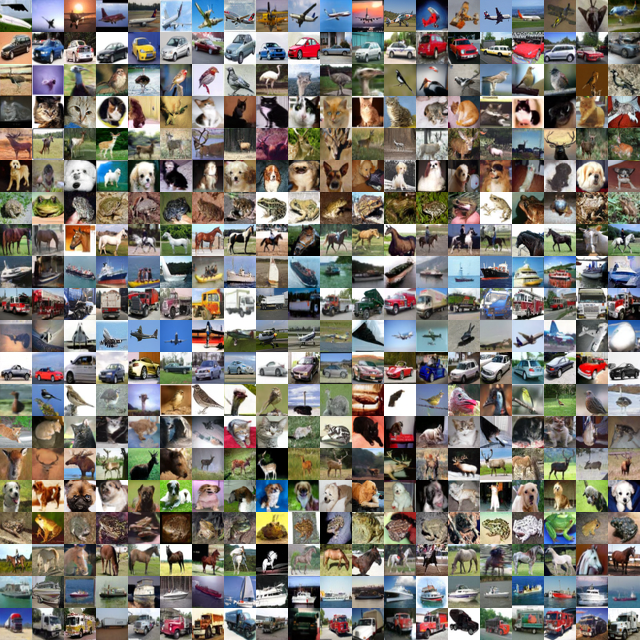
\includegraphics[width=\linewidth]{imgs/cond_CIFAR_FD.png}
    \caption{2-step samples from class-conditional ECM trained on CIFAR-10. Each row corresponds to a different class.}
    \label{fig:cifar-2-step}
\end{figure}

\begin{figure}[h!]
    \centering
    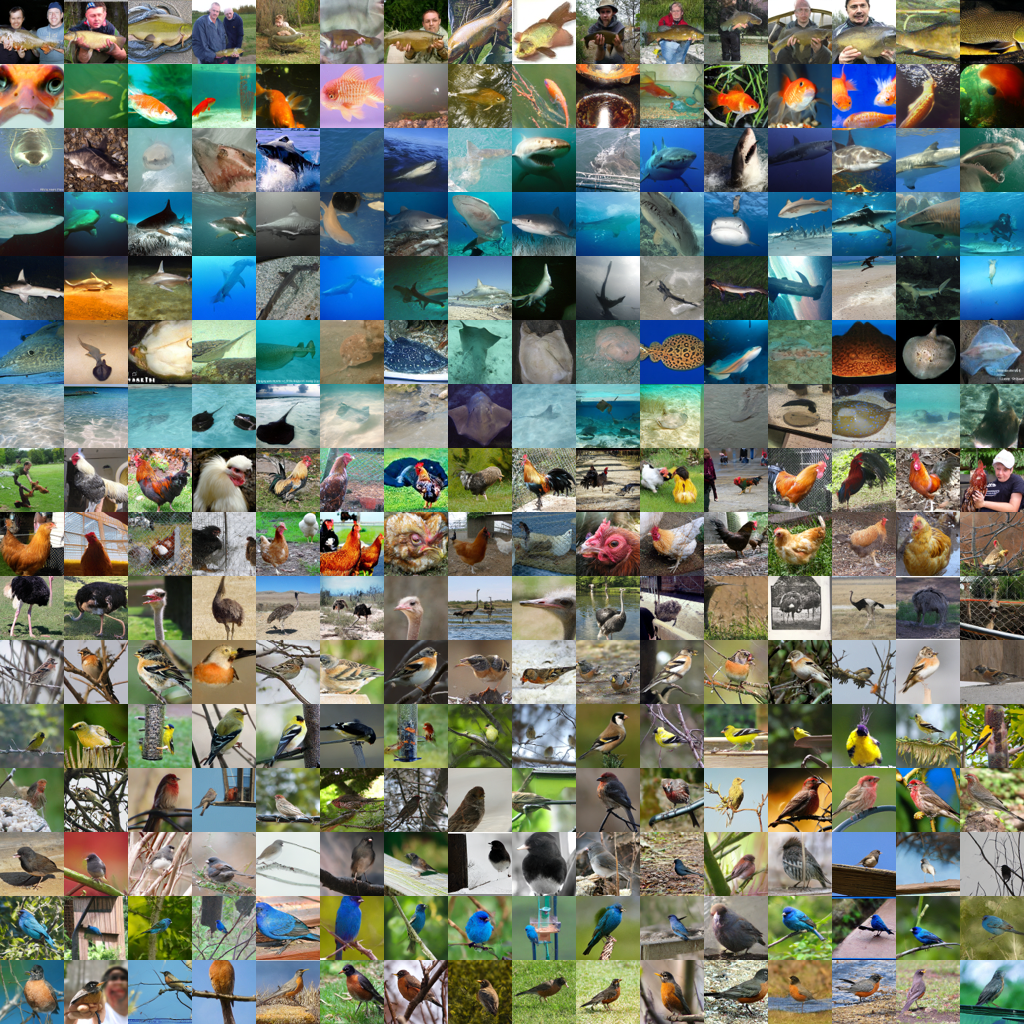
\includegraphics[width=\linewidth]{imgs/ECM-XL.png}
    \caption{2-step samples from class-conditional ECM-XL trained on \imgnet. Each row corresponds to a different class.}
    \label{fig:imagenet-2-step}
\end{figure}